\title{%
  \textbf{gdoc2latex}
  \linebreak \linebreak
  \large{Converts Google Docs files to LaTeX\\~\\~Your Name\\~Department of Something\\~University of Somewhere}
}\documentclass[12pt]{article}
\usepackage[a4paper,left=2.54cm,right=2.54cm,top=2.54cm,bottom=2.54cm]{geometry}

\usepackage[T1]{fontenc}
\usepackage[utf8]{inputenc}
\usepackage{lmodern}

\setlength\parindent{0em}
\usepackage{parskip}
\setcounter{tocdepth}{1}

\usepackage{hyperref}
\usepackage{graphicx}

\usepackage{titling}
\predate{}
\date{}
\postdate{}
\preauthor{}
\author{}
\postauthor{}

\begin{document}


\maketitle

\section{Usage}\label{id:h.9brqho78gj4b}

Here’s some content, originally written in Google Docs. It demonstrates using some of the features of gdoc2latex. It was downloaded with File > Download > Web page (.html).

{\centering \begin{figure}[h!]
  \centering
  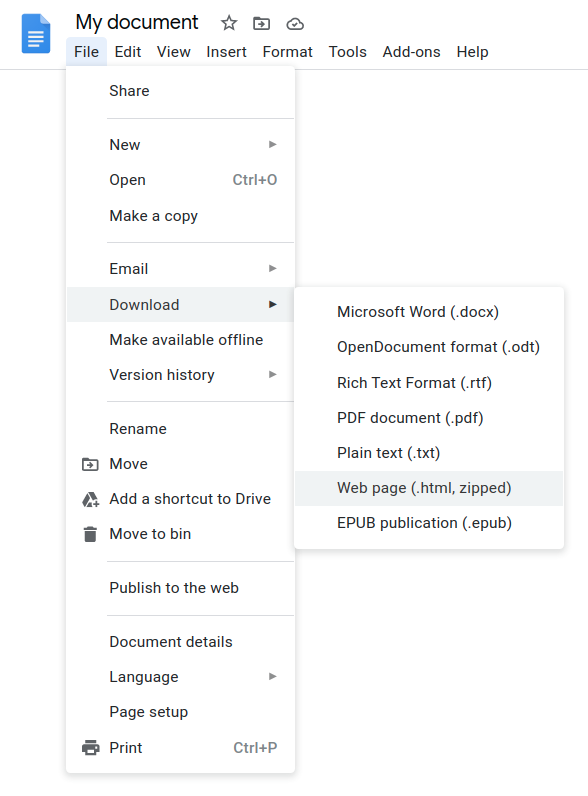
\includegraphics[width=0.5\linewidth]{images/image1.png}
  \caption{Downloading a document from Google Docs}
\end{figure} \par}

\section{Supported features}\label{id:h.3pfyws1px6lp}

Things like \textbf{bold} and \textit{italics} among other things are supported.

Other features include:

\begin{itemize}
  \item Lists
  \item \underline{Underline}
  \item References (use BibTeX in a Google Docs footnote)\cite{ref1}
  \item Footnotes\footnote{Like this! One limitation though, they can’t start with an @ symbol}
  \item Both \textsuperscript{superscript} and \textsubscript{subscript}
  \item Links to the \underline{\href{https://github.com/domdomegg/gdoc2latex}{web}}, to an \underline{\href{mailto:someone@example.com}{email address}} or \underline{\hyperref[id:h.9brqho78gj4b]{within a document}}
\end{itemize}

\bibliography{output}

\bibliographystyle{abbrvurl}

\end{document}